\chapter{角動量多重態、徑向運動與振子階梯}

\section{波函數的角度依賴}

中心力場中的粒子具有徑向座標和兩個角座標。經典力學中，
\begin{equation}
\mathbf L=\mathbf r\times\mathbf p
\end{equation}
是一個守恆向量。它的方向決定軌道平面，但軌道不一定是圓形。

量子力學中，粒子以
\begin{equation}
\Psi=\Psi(r,\theta,\phi),
\end{equation}
描述；角動量則與此波函數對角度的依賴有關。

在二維中，角動量只有一個分量，也就是繞垂直於平面的軸旋轉的生成元：
\begin{equation}
L_z=-i\hbar\frac{\partial}{\partial\theta}.
\end{equation}
本徵值為\(\hbar\ell\)的本徵函數滿足
\begin{equation}
-i\hbar\frac{\partial}{\partial\theta}\psi(r,\theta)
=\hbar\ell\,\psi(r,\theta).
\end{equation}
在這個方程中，座標\(r\)不受影響。方程的解具有以下形式：
\begin{equation}
\psi(r,\theta)=\chi(r)e^{i\ell\theta}.
\end{equation}
對於普通的單值軌道波函數，當\(\theta\to\theta+2\pi\)後回到同一點，要求\(\ell\)為整數。徑向因子\(\chi(r)\)可能影響能量，但不影響這個角動量本徵值。

三維的對應情形也能將徑向依賴與球面上的函數分離：
\begin{equation}
\Psi(r,\theta,\phi)=R(r)Y_{\ell m}(\theta,\phi).
\end{equation}
函數\(Y_{\ell m}\)稱為球諧函數。此處不需要它們的明確公式。旋轉作用在角度因子上，而徑向函數不變。

\section{有限角動量多重態}

角動量的分量滿足
\begin{equation}
\begin{aligned}
[L_x,L_y]&=i\hbar L_z,\\
[L_y,L_z]&=i\hbar L_x,\\
[L_z,L_x]&=i\hbar L_y.
\end{aligned}
\end{equation}
選取\(L_z\)的本徵態，
\begin{equation}
L_z|\ell,m\rangle=\hbar m\,|\ell,m\rangle,
\end{equation}
並定義
\begin{equation}
L_\pm=L_x\pm iL_y.
\end{equation}
由對易關係
\begin{equation}
[L_z,L_\pm]=\pm\hbar L_\pm
\end{equation}
可得
\begin{align}
L_z\bigl(L_\pm|\ell,m\rangle\bigr)
&=\bigl(L_\pm L_z+[L_z,L_\pm]\bigr)|\ell,m\rangle \\
&=\hbar(m\pm1)L_\pm|\ell,m\rangle.
\end{align}
因此，\(L_+\)會使\(m\)增加一，而\(L_-\)會使它減少一，除非所得向量為零。

有限多重態有一個最高態和一個最低態：
\begin{equation}
L_+|\ell,\ell\rangle=0,
\qquad
L_-|\ell,-\ell\rangle=0.
\end{equation}
\(+z\)與\(-z\)方向可以透過旋轉互相對應，因此有限譜以零為中心對稱。其取值為
\begin{equation}
m=-\ell,-\ell+1,\ldots,\ell-1,\ell,
\end{equation}
態的數目則是
\begin{equation}
2\ell+1.
\end{equation}
相鄰取值相差一，因此端點可以是整數或半整數。普通軌道球諧函數實現整數情形；抽象的角動量代數也容許半整數多重態。

\begin{classroomqa}
\lecturetimestamp{00:16:12}
\audiencequestion{角動量多重態能否包含無限多個態？}
\lecturerresponse{可以考慮這種可能性，但此處用不到。若態的其他性質保持不變，角動量通常會提高能量，因此討論有限能量態時，不必考慮角動量無限大的態。}
\end{classroomqa}

\section{\texorpdfstring{\(L^2\)}{角動量平方}的共同值}

測量角動量大小平方的算符是
\begin{equation}
L^2=L_x^2+L_y^2+L_z^2.
\end{equation}
階梯算符的有序乘積為
\begin{align}
L_-L_+
&=(L_x-iL_y)(L_x+iL_y) \\
&=L_x^2+L_y^2+i[L_x,L_y] \\
&=L_x^2+L_y^2-\hbar L_z.
\end{align}
因此，
\begin{equation}
L^2=L_z^2+\hbar L_z+L_-L_+.
\end{equation}
將這個恆等式作用於最高態。由於\(L_+|\ell,\ell\rangle=0\)，
\begin{align}
L^2|\ell,\ell\rangle
&=\left(L_z^2+\hbar L_z+L_-L_+\right)|\ell,\ell\rangle \\
&=\hbar^2\left(\ell^2+\ell\right)|\ell,\ell\rangle,
\end{align}
因此
\begin{equation}
L^2|\ell,\ell\rangle
=\hbar^2\ell(\ell+1)|\ell,\ell\rangle.
\end{equation}
角動量大小平方的本徵值不是\(\hbar^2\ell^2\)。多出的那一項源自角動量分量不對易。

多重態中的每個態都有相同的本徵值，不只有最高態如此。

\begin{classroomqa}
\lecturetimestamp{00:26:08}
\audiencequestion{這道證明其他態具有相同\(L^2\)的練習，究竟要說明什麼？}
\lecturerresponse{證明\(L^2\)與角動量的每個分量都對易，因此也與\(L_-\)對易。接著將\(L^2\)移過\(L_-\)：如果最高態的本徵值是\(\hbar^2\ell(\ell+1)\)，那麼下一個較低態的本徵值也相同。重複這個論證，就能將這個本徵值推到整個階梯上的所有態。}
\end{classroomqa}

確實，
\begin{equation}
[L^2,L_i]=0,
\qquad i=x,y,z,
\end{equation}
所以
\begin{equation}
[L^2,L_\pm]=0.
\end{equation}
例如，
\begin{align}
L^2\bigl(L_-|\ell,\ell\rangle\bigr)
&=L_-L^2|\ell,\ell\rangle \\
&=\hbar^2\ell(\ell+1)L_-|\ell,\ell\rangle.
\end{align}
依序往下可得
\begin{equation}
L^2|\ell,m\rangle
=\hbar^2\ell(\ell+1)|\ell,m\rangle
\end{equation}
對每個\(m=-\ell,\ldots,\ell\)皆成立。

將乘積以相反順序排列，也可得到等價的因式分解：
\begin{align}
L_+L_-
&=(L_x+iL_y)(L_x-iL_y) \\
&=L_x^2+L_y^2-i[L_x,L_y] \\
&=L_x^2+L_y^2+\hbar L_z,
\end{align}
因此
\begin{equation}
L^2=L_z^2-\hbar L_z+L_+L_-.
\end{equation}

\begin{classroomqa}
\lecturetimestamp{00:32:05}
\audiencequestion{能否使用\(L_+L_-\)，以相反順序將\(L_x^2+L_y^2\)因式分解？}
\lecturerresponse{可以。\(L_z\)項的正負號會反轉。依此順序，將恆等式作用於最低態；\(L_-\)會消去這個態，因此要用最低態，而不是最高態。同樣可得本徵值\(\hbar^2\ell(\ell+1)\)。}
\end{classroomqa}

因此，球諧函數滿足
\begin{align}
L^2Y_{\ell m}
&=\hbar^2\ell(\ell+1)Y_{\ell m}, \\
L_zY_{\ell m}
&=\hbar m\,Y_{\ell m}.
\end{align}
對每個軌道角動量值\(\ell=0,1,2,\ldots\)，都有\(2\ell+1\)個以\(m=-\ell,\ldots,\ell\)為標記的函數。

對於中心勢，
\begin{equation}
[H,L_i]=0.
\end{equation}
固定徑向能量本徵態和\(\ell\)後，若改變\(m\)並以\(L_\pm\)連接各態，能量不會改變。因此，每個這樣的徑向本徵態都形成一個維度為\(2\ell+1\)的磁量子數多重態。

以下顯示整數軌道角動量的階梯。\footnote{此圖依據講課影片\(00{:}35{:}53\)處可見的多重態草圖與算符恆等式重繪。}

\begin{figure}[htbp]
\centering
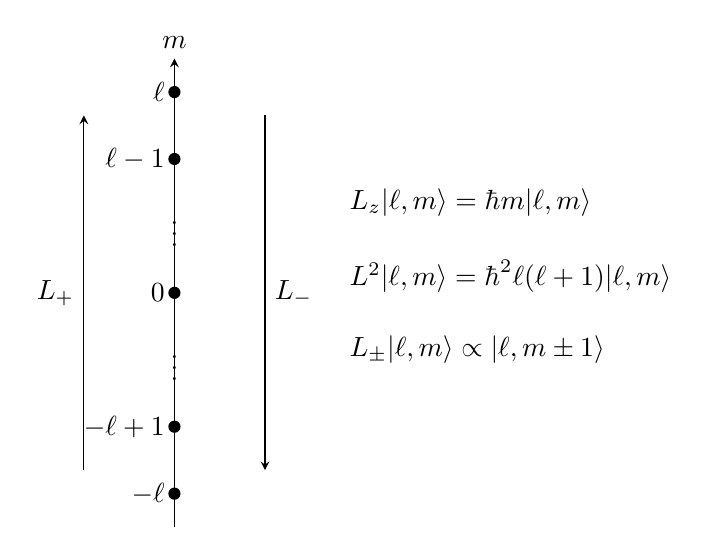
\begin{tikzpicture}[x=1cm,y=0.85cm,>=stealth]
\draw[->] (0,-3.5) -- (0,3.5) node[above] {$m$};

\fill (0,3) circle (2.2pt);
\fill (0,2) circle (2.2pt);
\fill (0,0) circle (2.2pt);
\fill (0,-2) circle (2.2pt);
\fill (0,-3) circle (2.2pt);

\node[left] at (0,3) {$\ell$};
\node[left] at (0,2) {$\ell-1$};
\node[left] at (0,0) {$0$};
\node[left] at (0,-2) {$-\ell+1$};
\node[left] at (0,-3) {$-\ell$};

\node at (0,1) {$\vdots$};
\node at (0,-1) {$\vdots$};

\draw[->] (-1.15,-2.65) -- (-1.15,2.65)
node[midway,left] {$L_+$};
\draw[->] (1.15,2.65) -- (1.15,-2.65)
node[midway,right] {$L_-$};

\node[anchor=west] at (2.1,1.35)
{$L_z|\ell,m\rangle=\hbar m|\ell,m\rangle$};
\node[anchor=west] at (2.1,0.25)
{$L^2|\ell,m\rangle=\hbar^2\ell(\ell+1)|\ell,m\rangle$};
\node[anchor=west] at (2.1,-0.85)
{$L_\pm|\ell,m\rangle\propto|\ell,m\pm1\rangle$};
\end{tikzpicture}
\caption{整數軌道角動量多重態。\(L_+\)和\(L_-\)會使\(m\)改變一，而\(L^2\)在整個多重態中保持為\(\hbar^2\ell(\ell+1)\)。}
\lectureframe{00:35:53}
\end{figure}

\section{中心力問題}

考慮
\begin{equation}
H=\frac{\mathbf p^2}{2m}+V(r),
\end{equation}
其中\(V\)只與到原點的距離有關。旋轉對稱性意味著角動量守恆。經典力學中，\(\mathbf L\)的大小和方向固定，因此軌道會保持在垂直於\(\mathbf L\)的平面內。軌道不一定是圓形，甚至不一定是封閉的。

選取座標，使這個經典軌道平面為\(xy\)平面，並將動量分解為徑向與切向分量：
\begin{equation}
\mathbf p^2=p_r^2+p_\theta^2.
\end{equation}
角動量的大小為
\begin{equation}
L=r p_\theta,
\end{equation}
因此切向分量的平方可寫成
\begin{equation}
p_\theta^2=\frac{L^2}{r^2}.
\end{equation}
哈密頓量便成為
\begin{equation}
H=\frac{p_r^2}{2m}+\frac{L^2}{2mr^2}+V(r).
\end{equation}
固定\(L\)後，這就成為一個以徑向座標為變數的一維問題，其有效勢為
\begin{equation}
V_{\mathrm{eff}}(r)=\frac{L^2}{2mr^2}+V(r).
\end{equation}
下方黑板上顯示的是徑向哈密頓量。\footnote{來源影格：\texttt{\detokenize{lecture_03_frame_02.png}}，講課影片時間\(00{:}47{:}15\)。}

\begin{figure}[htbp]
\centering
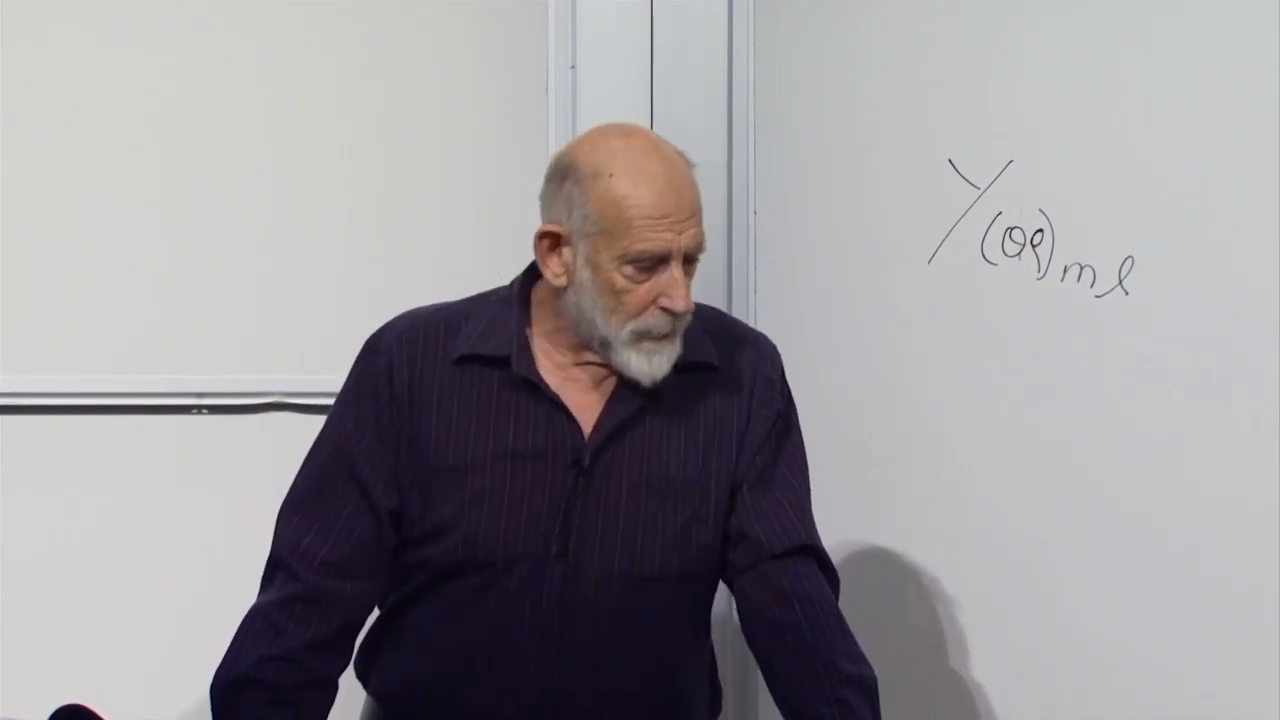
\includegraphics[width=0.9\linewidth]{lecture_03_frame_02.png}
\caption{固定經典角動量後，徑向哈密頓量包含徑向動能、離心項\(L^2/(2mr^2)\)和中心勢\(V(r)\)。}
\lectureframe{00:47:15}
\end{figure}

\(1/r^2\)項就是離心勢壘。粒子越接近原點，這一項越大，因此相應的力指向外。對於此處討論的類庫侖吸引勢，當\(L\neq0\)時，軌跡會繞著中心轉，而不會抵達中心。當\(L=0\)時，勢壘便不存在。

對於吸引庫侖勢，
\begin{equation}
V(r)=-\frac{\kappa}{r},
\end{equation}
在\(r\)較小處，離心項占優勢；庫侖項衰減得較慢，因此在\(r\)較大處占優勢。當\(L\neq0\)時，兩項之和有一個極小值。粒子在極小值處運動時，半徑保持不變，因此軌道是圓形。能量高於極小值、低於逃逸閾值的束縛運動，會在最小半徑和最大半徑之間來回振盪；在庫侖問題中，這就是橢圓軌道的徑向振盪。

\section{約化徑向方程}

量子力學中，具有確定軌道角動量的態，其角度部分是球諧函數。將分離變數後的態寫成
\begin{equation}
\Psi_{n_r\ell m}(r,\theta,\phi)
=\frac{u_{n_r\ell}(r)}{r}\,
Y_{\ell m}(\theta,\phi).
\end{equation}
角算符\(L^2\)的本徵值為
\begin{equation}
L^2Y_{\ell m}
=\hbar^2\ell(\ell+1)Y_{\ell m}.
\end{equation}
固定\(n_r,\ell\)後，將\(u_{n_r\ell}(r)\)簡寫為\(u(r)\)。剩下的約化徑向函數滿足方程
\begin{equation}
\begin{aligned}
&-\frac{\hbar^2}{2m}\frac{d^2u}{dr^2}
+\frac{\hbar^2\ell(\ell+1)}{2mr^2}u(r)\\
&\qquad+V(r)u(r)=E_{n_r\ell}\,u(r).
\end{aligned}
\end{equation}

\editorialnote{純粹的一維二階導數方程使用約化徑向函數\(u=rR\)。因此，講課方程中顯示的\(\psi(r)\)對應於\(u(r)\)；而在\(\Psi=R(r)Y_{\ell m}\)中，普通的徑向因子是\(R=u/r\)。採用這種寫法，可避免把\(-i\hbar\,d/dr\)當成三維徑向希爾伯特空間上的獨立厄米徑向動量算符。}

下方黑板上顯示的是約化徑向方程。\footnote{來源影格：\texttt{\detokenize{lecture_03_frame_03.png}}，講課影片時間\(00{:}54{:}32\)。}

\begin{figure}[htbp]
\centering
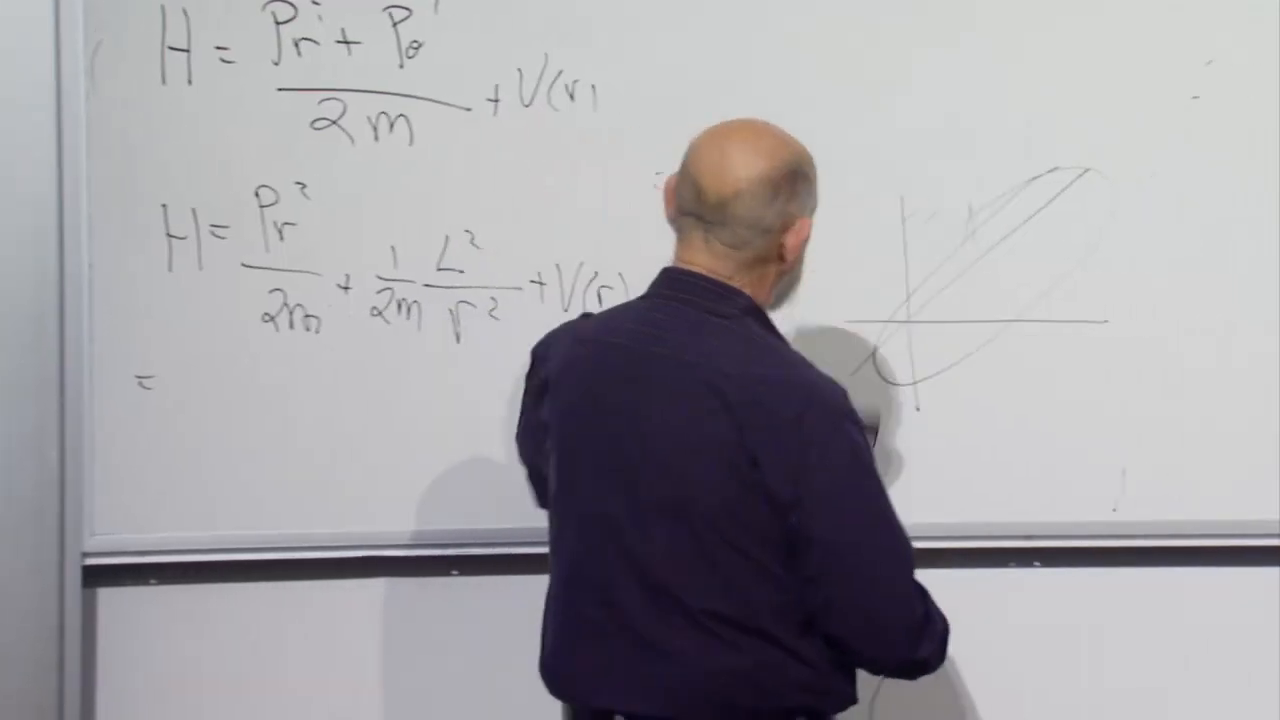
\includegraphics[width=0.9\linewidth]{lecture_03_frame_03.png}
\caption{固定\(\ell\)後，約化徑向波函數滿足一維Schr\"odinger方程，其中包含一個正比於\(\ell(\ell+1)/r^2\)的離心項。}
\lectureframe{00:54:32}
\end{figure}

三維角度結構的影響已濃縮在參數\(\ell\)中。徑向方程不含磁量子數\(m\)。

\begin{classroomqa}
\lecturetimestamp{00:55:34}
\audiencequestion{給定\(\ell\)後，\(2\ell+1\)個磁量子數態的能量是否相同？}
\lecturerresponse{是，只要徑向本徵態也固定即可。對每個選定的\(u_{n_r\ell}\)，所有\(m=-\ell,\ldots,\ell\)取值的態能量都相同，因為\(m\)不會出現在徑向方程中。同一\(\ell\)下，不同徑向本徵態的能量通常不同。}
\end{classroomqa}

\begin{classroomqa}
\lecturetimestamp{00:56:03}
\audiencequestion{為什麼可以用\(\hbar^2\ell(\ell+1)\)取代\(L^2\)？\(\ell\)與\(m\)的允許值有何關係？}
\lecturerresponse{數值\(\ell\)用來標記一個角動量多重態，也是該多重態中\(m\)的最大值。多重態中的每個態都具有相同的\(L^2\)本徵值\(\hbar^2\ell(\ell+1)\)，因此將此本徵值代入徑向方程。}
\end{classroomqa}

此處的論證不需要特殊函數解的明確形式。重要的是了解這些解如何排列。

\section{徑向節點與能階}

固定\(\ell\)後，約化徑向方程就是一個普通的一維本徵值問題。束縛態依內部節點數目排列。最低徑向態沒有內部節點，下一個有一個，再下一個有兩個。節點越多，波函數變化越快；變化越快，動量越大，因此動能也越大。

每個\(\ell\)取值都對應不同的徑向算符，因為離心項會隨\(\ell\)改變。因此，\(\ell=0,1,2,\ldots\)各自形成一系列徑向能階。隨角動量增加，正的離心項會使能階上移。固定\(\ell\)後，每個徑向本徵值都對應一個維度為
\begin{equation}
2\ell+1.
\end{equation}
的磁量子數多重態。\(\ell=0\)能階是單重態，\(\ell=1\)能階是三重態，\(\ell=2\)能階是五重態。這些簡併是旋轉對稱性所保證的；額外的對稱性也可能使不同\(\ell\)的態具有相同能量。

對於在\(r\)很大時滿足\(V(r)\to0\)的原子型勢，逃逸閾值依慣例取為\(E=0\)。能量為負的態構成離散束縛譜。在\(E=0\)及其以上則是散射連續譜。這項敘述取決於勢在\(r\)很大時的行為，因此不適用於具束縛作用的中心勢。

\section{特殊的庫侖簡併}

精確的非相對論庫侖勢還會使能階呈現另一種對應關係。最低的\(\ell=1\)徑向態與第一激發\(\ell=0\)態能量相同。下一個\(\ell=1\)態與第二激發\(\ell=0\)態能量相同，而最低的\(\ell=2\)態也與它們能量相同。這種模式會延續到更高的徑向與角動量能階序列。

\begin{classroomqa}
\lecturetimestamp{01:09:57}
\audiencequestion{這種額外的庫侖簡併是否代表另一種對稱性？}
\lecturerresponse{是。這是精確庫侖勢所具有的一種特殊額外對稱性。勢稍有變化，這種能階對應關係就會消失；此處不推導這種對稱性。}
\end{classroomqa}

由此得到的軌道殼層簡併度為
\begin{equation}
1,\qquad 4,\qquad 9,\qquad 16,\qquad \ldots
\end{equation}
這還未計入電子自旋。

\begin{classroomqa}
\lecturetimestamp{01:11:46}
\audiencequestion{這種簡併適用於氫原子，還是只適用於理想庫侖問題？}
\lecturerresponse{氫原子非常接近這種情形，但並非完全如此。相對論修正與原子核的有限大小都會擾動理想庫侖能階排列。}
\end{classroomqa}

點原子核產生精確的\(1/r\)勢。若原子核的電荷分布在一個小體積內，電子進入該體積時所受的勢就會略有不同；即使這個偏差很小，也會解除部分特殊簡併。

此處也尚未計入自旋。計入電子的兩種自旋態後，殼層態數加倍為
\begin{equation}
2,\qquad 8,\qquad 18,\qquad 32,\qquad \ldots
\end{equation}
這還未包含更完整原子理論所描述的進一步能階分裂。

\section{重新檢視笛卡兒座標下的方程}

徑向問題起始於三維定態Schr\"odinger方程：
\begin{equation}
\begin{aligned}
-\frac{\hbar^2}{2m}\nabla^2\Psi+V(r)\Psi&=E\Psi,\\
\nabla^2&=\frac{\partial^2}{\partial x^2}
+\frac{\partial^2}{\partial y^2}
+\frac{\partial^2}{\partial z^2},\\
r&=\sqrt{x^2+y^2+z^2}.
\end{aligned}
\end{equation}
改用徑向與角度座標，並選取\(L^2\)的本徵態。接著以\(\hbar^2\ell(\ell+1)\)取代\(L^2\)，便能將偏微分方程化約為前述的常微分徑向方程。

\begin{classroomqa}
\lecturetimestamp{01:16:42}
\audiencequestion{能否利用理想庫侖能譜的偏差來測定原子核大小？}
\lecturerresponse{無法只靠這種簡單比較來測定。其他修正大得多，必須先納入考量。此處提到原子核大小，是因為它是偏離點庫侖勢的一個直接例子。}
\end{classroomqa}

\begin{classroomqa}
\lecturetimestamp{01:17:09}
\audiencequestion{經典與量子角動量項的主要差異是什麼？}
\lecturerresponse{經典力學中，\(L^2\)是守恆向量大小的普通平方。在量子軌道多重態中，它的本徵值是\(\hbar^2\ell(\ell+1)\)，而不只是\(\hbar^2\ell^2\)。多出的那一項源自角動量分量不對易。}
\end{classroomqa}

\begin{classroomqa}
\lecturetimestamp{01:17:58}
\audiencequestion{束縛態波函數的支集是否為緊集？}
\lecturerresponse{不是。波函數會延伸到離中心任意遠處。對於此處討論的原子束縛態，波函數在遠處呈指數衰減，所以機率會變得微不足道，但在任何有限半徑之外都不會完全為零。}
\end{classroomqa}

\begin{classroomqa}
\lecturetimestamp{01:18:48}
\audiencequestion{當\(\ell=0\)使離心勢阱消失後，穩定點會如何變化？}
\lecturerresponse{離心勢壘與吸引力之間的競爭不再形成極小值。在點庫侖勢的理想化模型中，經典粒子會朝奇異中心運動。量子力學中，最低態不可能同時具有確定在中心的位置和零動量，因此最低態波函數會有有限的空間展寬。}
\end{classroomqa}

\editorialnote{對於正則的中心勢，經典零角動量軌跡可以穿過原點繼續運動。對於理想點庫侖勢，\(r=0\)則是碰撞奇點；若要延續經典軌跡，就需要另外訂定處理方式。}

經典力學的化約將單一軌道置於一個平面內，但量子波函數不能以同樣方式處理。量子軌道態遍布三維空間。完整的角動量算符為\(L^2=L_x^2+L_y^2+L_z^2\)，其本徵值保留了三維的結果\(\hbar^2\ell(\ell+1)\)。

\begin{classroomqa}
\lecturetimestamp{01:21:30}
\audiencequestion{經典軌道置於平面後，量子問題為何仍是三維的？}
\lecturerresponse{只有經典軌道被置於固定平面內：選取垂直於守恆角動量向量的座標即可做到。量子波函數仍佔據三維空間。其他角動量分量仍透過\(L^2\)保留下來，因此徑向方程包含\(\ell(\ell+1)\)，而不是只有單一分量的平方。}
\end{classroomqa}

\begin{classroomqa}
\lecturetimestamp{01:22:54}
\audiencequestion{每個量子問題都有升降算符嗎？}
\lecturerresponse{沒有。只有在一些特別有利的情況下才會出現升降算符。角動量問題是其中一例，諧振子問題則是另一例。諧振子的例子特別有用，因為穩定平衡附近的運動往往近似簡諧運動，包括有效勢極小值附近的小幅徑向振盪。}
\end{classroomqa}

此處先暫擱原子問題，接著以諧振子為例，說明如何利用階梯算符決定能譜。

\section{小振動與諧振子}

在穩定平衡附近，足夠小的位移往往會產生簡諧運動。非零角動量時的有效徑向勢就是一例：在勢阱底部附近，徑向運動近似為簡諧運動。

考慮質量為一的一維振子。令\(x\)表示偏離平衡位置的位移，並以\(k=\omega^2\)表示彈簧常數。經典哈密頓量為
\begin{equation}
H=\frac{p^2}{2}+\frac{\omega^2x^2}{2}.
\end{equation}
由哈密頓方程可得
\begin{equation}
\dot{x}=\frac{\partial H}{\partial p}=p,
\qquad
\dot{p}=-\frac{\partial H}{\partial x}=-\omega^2x,
\end{equation}
因此
\begin{equation}
\ddot{x}=-\omega^2x.
\end{equation}
所以\(\omega\)就是經典振盪頻率。

\section{因式分解與零點能}

量子力學中，
\begin{equation}
[x,p]=i\hbar.
\end{equation}
哈密頓量由平方項相加而成，因此可以嘗試以下因式分解：
\begin{align}
\frac{1}{2}(p+i\omega x)(p-i\omega x)
&=\frac{1}{2}\left(p^2+\omega^2x^2+i\omega[x,p]\right) \\
&=\frac{1}{2}\left(p^2+\omega^2x^2-\hbar\omega\right).
\end{align}
於是
\begin{equation}
H=\frac{1}{2}(p+i\omega x)(p-i\omega x)
+\frac{1}{2}\hbar\omega.
\end{equation}
加上的項\(\hbar\omega/2\)就是零點能。

經典力學中，最低能量會出現在\(x=p=0\)。量子力學中，沒有任何態能同時將位置和動量精確固定為零。此外，\(p^2/2\)與\(\omega^2x^2/2\)兩項都是正的，無法互相抵消。因此，基態能量必定不為零。

進行階梯算符計算時，可以先暫時略去共同的加性常數，最後再加回去。

\begin{classroomqa}
\lecturetimestamp{01:36:10}
\audiencequestion{零點能項為正，是否還能告訴我們其他事情？}
\lecturerresponse{振子哈密頓量是正算符：它是正平方項的總和，因此能量不可能為負。}
\end{classroomqa}

\section{振子階梯}

引入無因次算符。\footnote{在\(01{:}37\)--\(01{:}42\)附近的推導中，取\(\hbar=1\)。在這些歸一化定義中加回\(\hbar\)因子，使\(A_\pm\)成為無因次量，且其對易子為一。}
\begin{equation}
A_+=\frac{p+i\omega x}{\sqrt{2\hbar\omega}},
\qquad
A_-=\frac{p-i\omega x}{\sqrt{2\hbar\omega}}.
\end{equation}
它們互為厄米共軛：
\begin{equation}
A_+^\dagger=A_-.
\end{equation}
它們的對易子為
\begin{align}
[A_-,A_+]
&=\frac{1}{2\hbar\omega}
\left([p,i\omega x]+[-i\omega x,p]\right) \\
&=1.
\end{align}

定義
\begin{equation}
N=A_+A_-.
\end{equation}
哈密頓量便是
\begin{equation}
H=\hbar\omega\left(N+\frac{1}{2}\right).
\end{equation}
因此，求能譜就化約為求\(N\)的本徵值。

假設
\begin{equation}
N|n\rangle=n|n\rangle.
\end{equation}
與\(N\)的對易關係為\footnote{在\(01{:}45{:}37\)--\(01{:}48{:}10\)處的中間步驟，是直接根據已給出的關係\(N=A_+A_-\)和\([A_-,A_+]=1\)重建的。}
\begin{align}
[N,A_+]
&=A_+[A_-,A_+]=A_+, \\
[N,A_-]
&=[A_+,A_-]A_-=-A_-.
\end{align}
因此可得
\begin{align}
N\bigl(A_+|n\rangle\bigr)
&=(n+1)A_+|n\rangle, \\
N\bigl(A_-|n\rangle\bigr)
&=(n-1)A_-|n\rangle.
\end{align}
只要所得向量不為零，\(A_+\)就會使\(N\)的本徵值增加一，而\(A_-\)則會使它減少一。

算符\(N\)是非負的：
\begin{equation}
\langle\psi|N|\psi\rangle
=\langle\psi|A_+A_-|\psi\rangle
=\|A_-|\psi\rangle\|^2
\geq0.
\end{equation}
因此，降階過程不可能繼續到負本徵值。在底態\(|b\rangle\)處，這個過程必須終止：
\begin{equation}
A_-|b\rangle=0.
\end{equation}

對歸一化本徵態而言，階梯上的係數由範數決定：
\begin{align}
\|A_-|n\rangle\|^2
&=\langle n|A_+A_-|n\rangle=n, \\
\|A_+|n\rangle\|^2
&=\langle n|A_-A_+|n\rangle=n+1.
\end{align}
因此可以選擇相位，使得
\begin{equation}
A_-|n\rangle=\sqrt{n}\,|n-1\rangle,
\qquad
A_+|n\rangle=\sqrt{n+1}\,|n+1\rangle.
\end{equation}

\begin{classroomqa}
\lecturetimestamp{01:52:42}
\audiencequestion{如果\(A_-\)使一個態降低，而\(A_+\)又把它升回去，那麼\(A_+A_-\)怎麼會得到本徵值\(n\)？}
\lecturerresponse{階梯算符作用時會帶有歸一化因子。先作用\(A_-\)會帶來因子\(\sqrt n\)；接著對所得態作用\(A_+\)，又會帶來因子\(\sqrt n\)。兩者相乘就是\(n\)。}
\end{classroomqa}

確實，
\begin{equation}
A_+A_-|n\rangle
=\sqrt n\,A_+|n-1\rangle
=n|n\rangle.
\end{equation}

\begin{classroomqa}
\lecturetimestamp{01:55:52}
\audiencequestion{\(N\)的最低本徵值必須是零嗎？它也可能是正值嗎？}
\lecturerresponse{最低本徵值必定是零，而\(N\)的譜由非負整數構成。此處尚未證明這個端點結果。}
\end{classroomqa}

\editorialnote{令\(|b\rangle\)為最低態。由於降階過程必須終止，\(A_-|b\rangle=0\)。因此立即可得\(N|b\rangle=A_+A_-|b\rangle=0\)，所以\(N\)的最低本徵值為零。}

從這個最低態出發，作用\(A_+\)可得
\begin{equation}
n=0,1,2,\ldots.
\end{equation}
加回零點能這個加性項後，振子的能量為
\begin{equation}
E_n=\hbar\omega\left(n+\frac{1}{2}\right),
\qquad n=0,1,2,\ldots.
\end{equation}

接下來會進一步發展振子代數，並用它來求解其他量子問題。